\documentclass{article}
\usepackage{amsmath}
\usepackage{amssymb}
\usepackage{hyperref}
\usepackage{xcolor}
\usepackage{graphicx}

\title{A Modest (Tokenomics) Proposal}
\date{250305}
\author{}

\begin{document}

\maketitle

\section{Goals}
\begin{itemize}
    \item HYPR provides genuine utility to users
    \item HYPR has long-term incentives to keep demand in long-term
    \item HYPR allows user to be involved in useful DAO governance
\end{itemize}

\section{Voting Power}

Voting power depends on two parameters: $n$, the number of HYPR tokens locked, and $t$, the remaining period tokens are locked for (in weeks).
Token supply is denoted $S$ (it is $10^8 = 100\_000\_000$).
Max lock time is denoted $T$ (it is some small single-digit number of years).
The voting power of a wallet is denoted $V(n, t)$.
\begin{equation}
V(n, t) = (an - bn^2) \cdot (ct - dt^2)
\end{equation}

The parameters $a$, $b$, $c$, $d$, all greater than or equal to $0$, are chosen such that voting power is a strictly monotonically-increasing function of $n$ and $t$ (i.e. it only ever increases as $n$ and $t$ increase).
This leads to the following requirements for the parameters:
\begin{align}
a &> 2b \cdot n_m\\
c &> 2d \cdot T
\end{align}

where $n_m$ is the maximum number of tokens that a single wallet can lock.
$n_m$ can reasonably be set to $S$.

\begin{figure}[h]
    \centering
    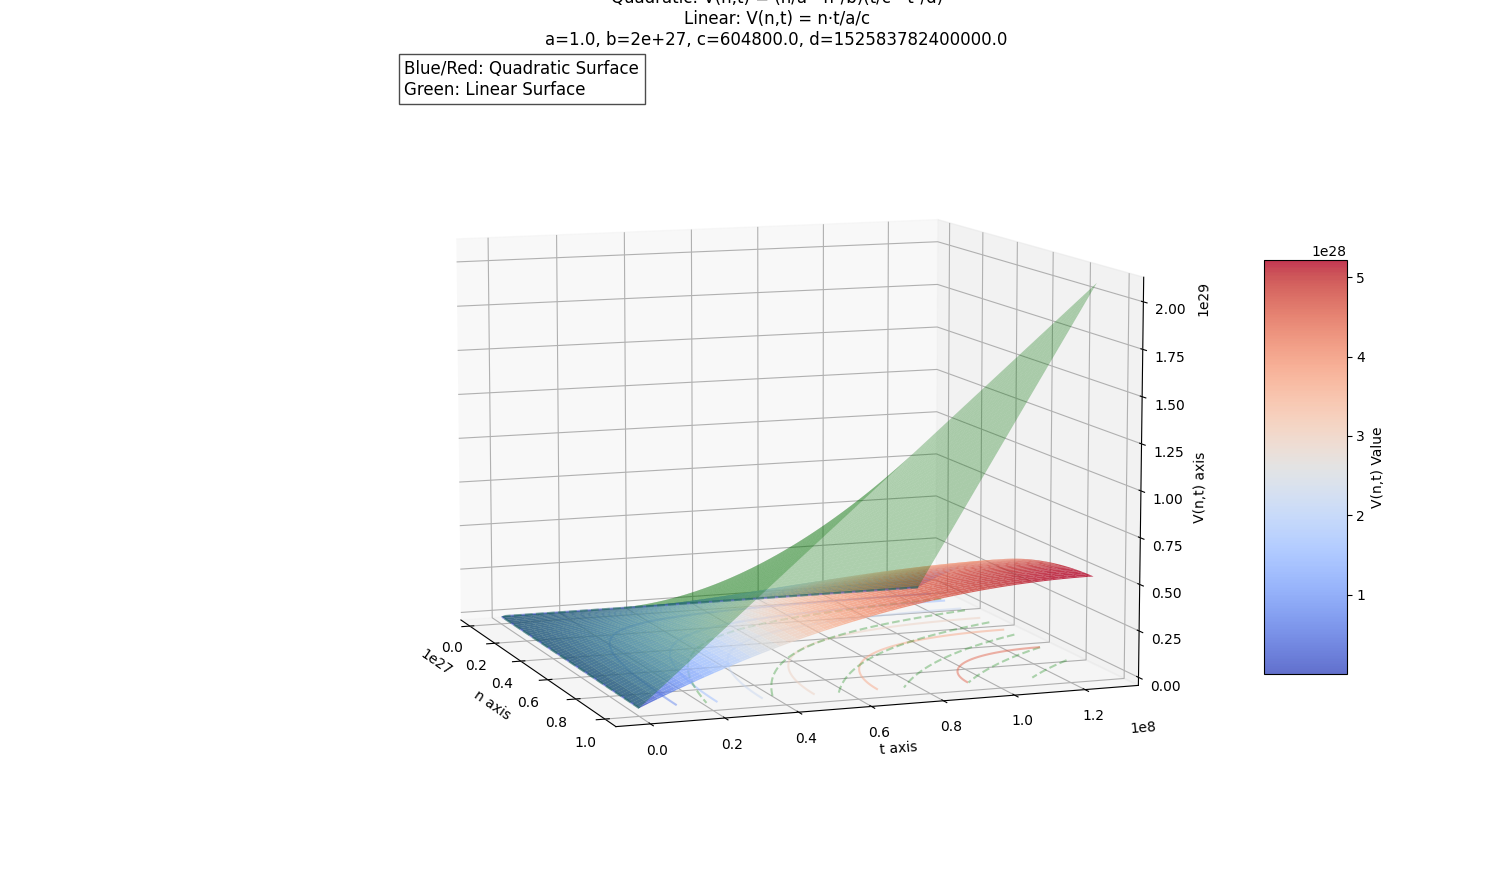
\includegraphics[width=0.7\textwidth]{voting-power-surface.png}
    \caption{An example of $V(n, t)$ with $a = c = 1$ and $b = d = 0.05$ compared with the ``linear surface'' $ab * nt$.}
    \label{fig:example-image}
\end{figure}

If $n$ or $t$ is $0$, $V$ is $0$.
The role of the parameters $b$ and $d$ is to make the voting power sub-linear in $n$ and $t$, respectively.
This means that:
\begin{itemize}
    \item A whale who locks a large amount of tokens does not dominate voting to the same degree as they would in the linear case (e.g. if one user owns 51\% of the tokens, locking them all will result in less than 51\% of the possible voting power).
    \item Locking for the maximum period gets less than double locking for half the maximum period.
    \item The sublinearity can be tuned by changing the value of $b$ and $d$.
      As $b$ or $d$ tends to $0$, the voting power tends to linear in $n$ or $t$ respectively.
\end{itemize}

Voting power decreases as time passes.
Say initial lock is for 100 HYPR for 52 weeks.
Initial voting power is then
\begin{equation}
V(n=100, t=52) = (a\cdot 100 - b\cdot 100^2) \cdot (c\cdot 52 - d\cdot 52^2)
\end{equation}

After one week has past, $t$ declines to $51$.
Each subsequent week, voting power of the locked tokens decreases, until it eventually reaches $0$.

A locked token position can be modified in three ways:
\begin{enumerate}
    \item Token lock can be extended.
       For example, say 100 tokens were locked for 52 weeks and 20 have passed, leaving 32 weeks remaining in the lock.
       The user can extend the lock to 52 weeks once again, extending the lockup period by an additional 20 weeks, and bringing voting power up to its original value.
    \item Tokens may be added.
       For example, say 100 tokens we locked for 52 weeks and 20 have passed, leaving 32 weeks remaining in the lock.
       10 additional tokens might be added, leading to a locked set of 110 tokens for 32 weeks.
    \item Tokens within the locked set may be registered, see \hyperref[sec:registration]{Registration discussion below}.
\end{enumerate}

Note that locked tokens cannot be unlocked until the locked time has passed!

\subsection{Voting Power Open Questions}
\begin{itemize}
    \item Token supply, $S$, is fixed at $10^8 = 100\_000\_000$ at launch.
      Will more tokens ever be minted?
    \item What is the max lock time, $T$?
\end{itemize}

\section{Registration}\label{sec:registration}

Tokens that are locked can be registered.
Registration can occur on either all locked tokens (that have not yet been registered) or a subset.
Registration points those tokens at a name-key on the Hypermap.

Registration power has a similar form to voting power with the number of locked tokens allocated to the registration, $r_{node}$, where $_{node}$ denotes the name-key in the Hypermap.
Thus, if we denote registration power $R(r_{node}, t)$, then we can write
\begin{equation}
R(r_{node}, t) = V(n=r_{node}, t)
\end{equation}

Registering tokens to a $_{node}$ is similar in some ways to locking tokens, and different in others.

Similar:
\begin{itemize}
    \item Registered tokens cannot be unregistered until the locked time has passed.
    \item Additional locked tokens can be added to a $_{node}$.
\end{itemize}

Different:
\begin{itemize}
    \item Increasing the locked time increases the registration time as well.
\end{itemize}

\section{Voting in DAO Governance}

A proposal has a closing time associated with it.
Voters cast votes.
Voting power of voters is calculated at closing time, and the proposal passes or fails.
Voters and their voting power, as well as the result of the vote, is recorded.

\section{Governance Participation Rewards}

Governance participation incentives are distributed quarterly: 2\% of the incentive treasury per quarter.
For each proposal, a user $i$ that participates in that vote gets an award $A_i$ that is a fraction of the incentives dedicated to that vote equal to
\begin{equation}
A_i = \frac{V_i}{\sum_i V_i}
\end{equation}

If no votes occur in a quarter, no incentives are distributed.
If multiple votes occur in a quarter, the incentives are split amongst them based on the total voting power that participated in each vote.
Denote the $j$th vote in a quarter $V^{j}$.
Then the fraction of quarterly incentives allocated to a specific vote $j$, $F^{j}$ is
\begin{equation}
F^{j} = \frac{\sum_i V^{j}_i}{\sum_i \sum_j V^{j}_i}
\end{equation}

and so the total award of a user in a multi-vote quarter looks like
\begin{equation}
A_i = \sum_j \left[F^{j} \cdot \frac{V^{j}_i}{\sum_i V^{j}_i}\right]
\end{equation}

\section{Vesting}

Vesting tokens cannot do anything except be fractionally claimed, depending on the percentage of the vesting time that has passed.
Thus, they cannot participate in locking, governance, registration.
They cannot be transferred.

There are two reasons that vesting tokens cannot do anything:
\begin{enumerate}
    \item Simplicity.
       Vesting tokens will only exist for the start of the network.
       There should not be logic for them that lives forever in locking, governance, registration contracts.
    \item Giving community members a headstart on governance and incentive rewards.
       Investors and team members will only be able to access a fraction of their tokens -- the ones that have already vested -- and thus will not be able to control governance due to their outsized ownership in early days.
       This also gives community members a chance to acquire a larger fraction of the governance rewards, improving the distribution of tokens to the community.
       Investors and team members have been of fundamental importance to the project and will continue to be so, but establishing an involved and aligned community is of the utmost importance for Hyperware to succeed.
\end{enumerate}

\end{document}
